\chapter{Image Processing}

\section{Image Features}
\par Image features are analogous to image properties. Since spam images are generated by computer, properties of spam images vary a lot from natural/ham images. For instance change in brightness in natural images is very high compared to that of spam images. Using advanced image processing techniques many such properties can be extracted from images.  A total of 41 features were collected  of which 21 are based on previous research ~\cite{6}. Table \ref{table:feature_set} gives a brief overview of all the features. These features can be loosely classified in 5 domains. 

\begin{itemize}
	\item Metadata Features: Properties like image size, height, width, aspect ratio, compression ratio, bit depth, image name, etc. are the basic set of properties of an image. A certain anomaly can be seen in computer generated images versus natural images. We used compression ratio and aspect ratio as 6 features.
	\item Color Features: Different histograms convey different properties of an image. 
	\begin{itemize}
		\item Color Histogram: A color histogram extracts the usage of Red, Green, Blue colors. Normally in a spam image, very few colors are used compared to natural images. Along with color histogram, RGB histograms can also be quantized and used for classification. Fig. \ref{fig:color_histograms}. compares the RGB channels of ham and spam images.
		
		 \begin{figure}[h]
		
			\begin{subfigure}{0.5\textwidth}
				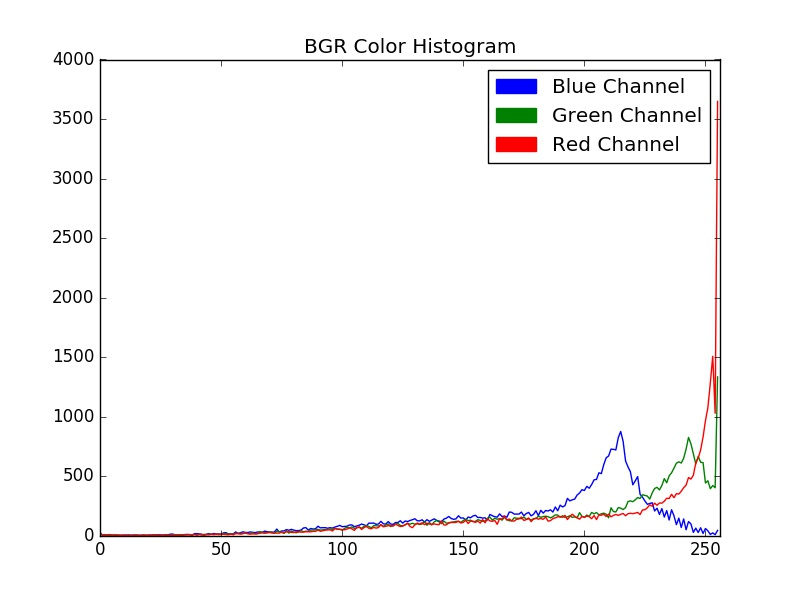
\includegraphics[width=0.9\linewidth]{images/ham_histogram} 
				\caption{Ham}
				\label{fig:ham_color_histograms}
			\end{subfigure}
			\begin{subfigure}{0.5\textwidth}
				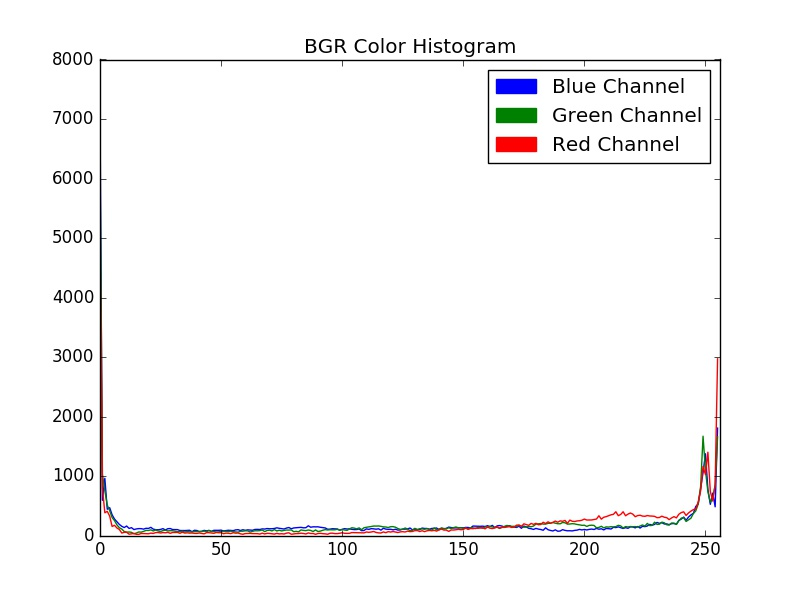
\includegraphics[width=0.9\linewidth]{images/spam_histogram}
				\caption{Spam}
				\label{fig:spam_color_histograms}
			\end{subfigure}
			\caption{RGB Channels of Color Histogram}
			\label{fig:color_histograms}
		\end{figure}
	
	
	
	
		\item Reg, Green, Blue Histograms: Mean, Variance, Skew and Kurtosis of each of these 3 histograms is calculated. All combined 12 features are extracted from the 3 histograms. 
		\item Hue, Saturation and Value (HSV) Histogram: HSV Histogram captures the following 3 aspects of the colors of  an image. 
		\begin{itemize}
			\item Hue: It defines how close the color is to red. Hue is measured between 0 to 1; 0 being red.
			\item Saturation: It defines how pure the color is. Higher values of saturation correspond to deeper/richer colors. While corresponds to 0 saturation.
			\item Intensity/Value: Intensity defines brightness. Higher values of intensity correspond to white.
		\end{itemize}
		\item Hue, Saturation, Intensity Histograms: Mean, skew, variance nd kurtosis of each of these histograms are captured. This adds up to 12 features extracted from the 3 features.  Fig. \ref{fig:hsv_histograms}. compares the HSV channels of ham and spam images.
		
		\begin{figure}[h]
			
			\begin{subfigure}{0.5\textwidth}
				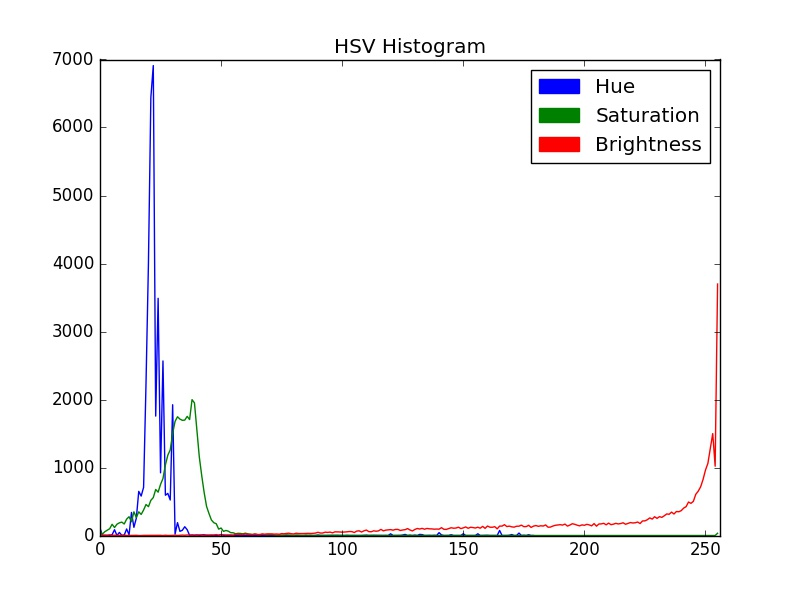
\includegraphics[width=0.9\linewidth]{images/ham_HSV_histogram} 
				\caption{Ham}
				\label{fig:ham_hsv_histograms}
			\end{subfigure}
			\begin{subfigure}{0.5\textwidth}
				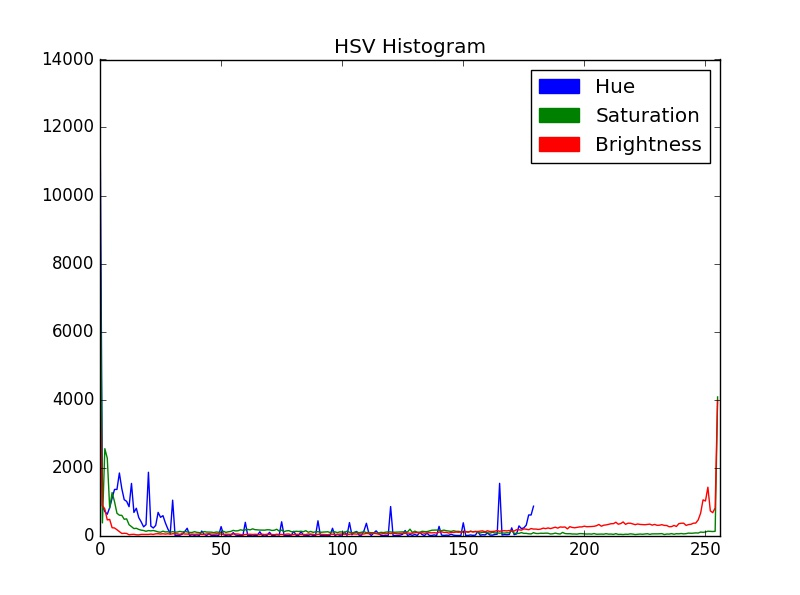
\includegraphics[width=0.9\linewidth]{images/spam_HSV_histogram}
				\caption{Spam}
				\label{fig:spam_hsv_histograms}
			\end{subfigure}
			\caption{HSV Channels of HSV Histogram}
			\label{fig:hsv_histograms}
		\end{figure}
	\end{itemize}
	\item Texture Features:
	\begin{itemize}	
		\item Local Binary Pattern (LBP) Histogram: This histogram is commonly used for texture classification. For each pixel, LBP helps quantify how similar or different each pixel is from its neighboring pixels. Spam images have relatively less information in this histogram.
	\end{itemize}
	
	\item Shape Features:
	\begin{itemize}	
		\item Histogram of Oriented Gradients: This histogram is commonly used for object detection. It describes how the intensity of gradients change in the image. 
		\item Edges: Edges mark the change in contrast. Edge detection highlights boundaries of features in an image~\cite{6}. Fig. ~\ref{fig:cannyEdges}. shows canny edge detector output on a spam image and a ham image. Spam images in general contain a lot of text, resulting in an increased number of edges than ham images. Another observation we can make by looking at the images is that edges in spam images are smaller compared to that in ham images. Number of edges and average edge length have been considered as 2 features.
		\begin{figure}[h]
			\centering
			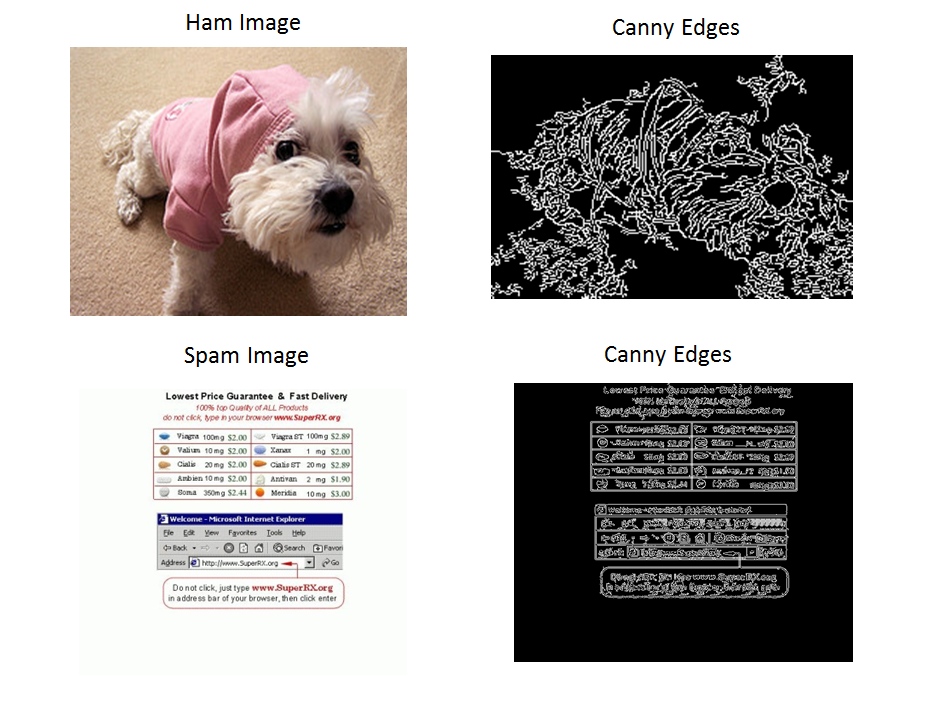
\includegraphics[width=0.75\textwidth]{images/cannyEdges.PNG}
			\caption{Canny Edge}
			\label{fig:cannyEdges}
		\end{figure}   
	\end{itemize}
	
	\item Noise Features:
	\begin{itemize}
		\item Entropy of Noise: Amount of noise in a spam image is less than a normal image. Entropy of noise histogram is measured as a feature.
		\item Signal to Noise Ratio (SNR): For this paper SNR is the ratio of mean and standard deviation in grayscale image's histogram.  	
	\end{itemize}
\end{itemize}


\begin{table}[htb]
	\centering
	\caption{Feature set}
	\begin{tabular}{ |c|c|c| } 
		\hline
		Feature Domain & Feature & Description \\
		\hline
		\multirow{6}{4em}{Metadata Features} & Height & Height of the image \\
		&	Width & Width of the image \\ 
		&	Aspect Ratio & Ratio of height and width \\ 
		&   Compression Ratio & How compressed is the image \\ 
		&   File Size & Size on disk\\ 
		&   Image Area & Area of the image\\ 
		\hline
		\multirow{26}{4em}{Color Features} & entr-color & Entropy of color histogram\\
		&	r-mean & Mean of the red channel histogram\\ 
		&	g-mean & Mean of the green channel histogram\\ 
		&   b-mean & Mean of the blue channel histogram \\ 
	
		&	r-skew & Skew of the red channel histogram\\ 
		&	g-skew & Skew of the green channel histogram\\ 
		&   b-skew & Skew of the blue channel histogram \\ 
		
		&	r-var & Variance of the red channel histogram\\ 
		&	g-var & Variance of the green channel histogram\\ 
		&   b-var & Variance of the blue channel histogram \\ 
		
		&	r-kurt & Kurtosis of the red channel histogram\\ 
		&	g-kurt & Kurtosis of the green channel histogram\\ 
		&   b-kurt & Kurtosis of the blue channel histogram \\ 
		
		&   entr-hsv & Entropy of HSV Histogram \\
		&	h-mean & Mean of the hue channel of hsv histogram\\ 
		&	s-mean & Mean of the saturation channel of hsv histogram\\ 
		&   v-mean & Mean of the brightness channel of hsv histogram \\ 
	
		&	h-var & Variance of the hue channel of hsv histogram\\ 
		&	s-var & Variance  of the saturation channel of hsv histogram\\ 
		&   v-var & Variance of the brightness channel of hsv histogram \\ 

		&	h-skew & Skew of the hue channel of hsv histogram\\ 
		&	s-skew & Skew of the saturation channel of hsv histogram\\ 
		&   v-skew & Skew of the brightness channel of hsv histogram \\ 
	
		&	h-kurt & Kurtosis of the hue channel of hsv histogram\\ 
		&	s-kurt & Kurtosis of the saturation channel of hsv histogram\\ 
		&   v-kurt & Kurtosis of the brightness channel of hsv histogram \\ 
		\hline
		\multirow{1}{4em}{Texture Features} & lbp & Entropy of Local Binary Patterns histogram \\
		\hline
		\multirow{3}{4em}{Shape Features} & entr-hog & Entropy of Histogram of gradients\\
		&	edges & Total number of edges in an image\\ 
		&	avg-edge-length & Average edge length \\ 
		\hline
		\multirow{3}{4em}{Noise Features} & snr & Signal to Noise Ratio\\
		& entr-noise & Entropy of noise\\ 
		\hline
			
	\end{tabular}
	\label{table:feature_set}
\end{table}



\section{Feature Selection}

Once features have been extracted, these features have to be quantized. This process can be coined as preparing the data. Machine Learning algorithms require input in the form of feature vectors, wherein each feature is a number. Hence image features like canny edges, histograms, etc. have to be converted to numbers. Various statistical techniques like entropy of histograms, mean, variance, kurtosis, extracting number of edges from canny edge image, etc. are used. 

\par Once feature vectors are constructed, multiple experiments can be conducted to select a subset of features to achieve greater accuracy.
